\documentclass[conference]{IEEEtran}
\IEEEoverridecommandlockouts
\usepackage{cite}
\usepackage{amsmath,amssymb,amsfonts}
\usepackage{graphicx}
\graphicspath{{../figs/}}
\usepackage{textcomp}
\usepackage{xcolor}
\usepackage{booktabs}
\usepackage{url}
\renewcommand{\topfraction}{0.95}
\renewcommand{\bottomfraction}{0.95}
\renewcommand{\textfraction}{0.05}
\renewcommand{\floatpagefraction}{0.9}
\renewcommand{\dbltopfraction}{0.95}
\renewcommand{\dblfloatpagefraction}{0.9}
\def\BibTeX{{\rm B\kern-.05em{\sc i\kern-.025em b}\kern-.08em
    T\kern-.166em\lower.7ex\hbox{E}\kern-.125emX}}

\begin{document}

\title{Clause-Activation Signatures (CAS) for Attack-Family Attribution in IoMT using Tsetlin Machines}

\author{{\small Rakesh Reddy Yakkati, Per-Arne Andersen, Lei Jiao, Rishad Shafik, Alex Yakovlev, and Ole-Christoffer Granmo}
\thanks{Supported by the Research Council of Norway (SecureIoTM, grant 342167, TEKNOLOGIKONVER), with support from CAIR at the University of Agder, S\o rlandet Hospital Trust, and Newcastle University.}%
\thanks{R. R. Yakkati, L. Jiao, and O.-C. Granmo: Dept. of ICT, University of Agder, Grimstad, Norway; P.-A. Andersen: Dept. of Information Systems, University of Agder, Kristiansand, Norway; R. Shafik: Dept. of Microelectronic Systems, Newcastle University, UK; A. Yakovlev: Electrical and Electronic Engineering, School of Engineering, Newcastle University, Newcastle upon Tyne NE1 7RU, UK. Contact: rakeshry@uia.no.}}

\maketitle

\begin{abstract}
Intrusion detection in the Internet of Medical Things (IoMT) must
identify attack families and provide evidence that analysts can inspect.
We introduce Clause-Activation Signatures (CAS), which extract signed
clause evidence from a trained weighted Tsetlin Machine (TM).
Complementary-pairs stability selection identifies repeatedly selected
clauses, and averaged coefficient signs distinguish supporting from
opposing evidence. Optional weight-based pruning reduces the candidate
pool. We evaluate on capped CICIoMT2024 WiFi/MQTT data. The training
set is partitioned three ways. The TM is fitted on the first partition,
signatures are extracted on the second, and the operating point is
chosen on the third. The second partition is withheld from TM training.
The test set is read once. Across three seeds the full 2,400-clause TM
reaches macro-F1 $0.6660\pm0.0125$. At $\pi_{\mathrm{thr}}=0.8$ CAS
retains 149 clauses and reaches $0.6660\pm0.0316$. At
$\pi_{\mathrm{thr}}=0.9$ it retains 126 clauses and reaches
$0.6599\pm0.0371$. The signature is therefore 16 to 19 times smaller
than the clause pool, with no measurable change in macro-F1. Replacing
the clause pool with the 154 input literals under the same readout
drops macro-F1 to $0.5876\pm0.0112$. A decision tree, an $\ell_1$
linear model, XGBoost and a random forest on the same literals span
$0.6551$ to $0.6948$. CAS is therefore competitive with these models
rather than more accurate, and its contribution is the compactness of
the evidence it exposes. We derive a sufficient condition for pruning to
preserve TM predictions and clarify the scope of stability-selection
error control. Reliance on one capped dataset requires independent
validation.
\end{abstract}

\begin{IEEEkeywords}
attack attribution, intrusion detection, interpretable machine learning,
IoMT, stability selection, Tsetlin Machine
\end{IEEEkeywords}

\section{Introduction and Related Work}
Attack-family attribution identifies the type of malicious traffic,
helping analysts prioritize alerts and choose appropriate responses in
the Internet of Medical Things (IoMT). Neural-network approaches address
this task through multiclass intrusion classification; for example,
Yin et al.~\cite{yin2017} used recurrent neural networks to distinguish
normal traffic and four attack categories on NSL-KDD. However, these
predictions do not directly expose human-readable decision rules.
Post-hoc methods such as SHAP and LIME explain feature contributions to
intrusion predictions~\cite{xaiids2025}, but a predicted label alone
still lacks explicit evidence explaining why one attack family is
favored over another.

The Tsetlin Machine (TM) learns conjunctive rules over Boolean
literals~\cite{granmo2018}, while weighted variants assign learned
weights to these clauses~\cite{phoulady2020}. Its rule-based structure
makes the conditions contributing to a class vote available for
inspection. Previous studies have used TM rules for interpretable
intrusion detection~\cite{abeyrathna2020}, including recent IoMT
applications that examine clause activations and class
votes~\cite{jaiswal2026iomt}. These studies motivate
using the detector's own Boolean clauses as evidence for attack-family
attribution. A trained clause pool, however, is not automatically a compact class
signature. It can contain redundant rules, and a clause's importance
to the TM vote need not reflect its usefulness for distinguishing one
family from the others. A useful signature should expose both
supporting and opposing evidence, remain reusable across flows, and
keep each score traceable to the clauses that fired. Compactness and
repeatable selection must therefore be assessed alongside predictive
performance, rather than treated as sufficient evidence of explanation
quality.

We introduce Clause-Activation Signatures (CAS), which apply
complementary-pairs stability selection
(CPSS)~\cite{meinshausen2010,shah2013} to a frozen clause pool and retain
signed evidence for and against each class. Optional weight-based
pruning reduces the candidate pool before signature extraction, and
normalized evidence matching produces the attribution score. Our contributions are:
\begin{itemize}
\setlength{\itemsep}{0pt}
\item A signed clause-based attribution layer using CPSS and normalized
supporting and opposing evidence.
\item A sufficient margin condition for prediction-preserving TM pruning
and an explicit account of the scope of CPSS error control.
\item A three-seed evaluation of full and pruned pools for multiclass
attribution, including non-TM reference models, a literal-substrate
ablation, sign ablation, and signature sizes.
\end{itemize}

\section{Method: Clause-Activation Signatures}
\subsection{Booleanisation and Weighted TM}
\label{sec:bool}
Figure~\ref{fig:cpss} summarizes the pipeline. Training-fitted quantile
bins encode numeric features as cumulative thermometer bits; non-finite
values are replaced with the finite training maximum. TMU~\cite{tmu}
supplies literal negation internally. For $C$ classes and $K$ clauses
per class, the trained pool produces Boolean activations
$z_{c,j}(x)$ and signed class sums
\begin{equation}
 f_c(x)=\sum_{j=1}^{K} w_{c,j}z_{c,j}(x),\qquad
 \hat y_{\mathrm{TM}}(x)=\arg\max_c f_c(x).
 \label{eq:tm}
\end{equation}
Flattening class and clause indices gives the activation matrix
$Z\in\{0,1\}^{n\times p}$, initially with $p=CK$.

\begin{figure*}[!t]
\centering

\includegraphics[width=1\textwidth]{fig_cpss_protocol.png}
\caption{CAS pipeline with optional pruning, CPSS, and signed attribution.
Disjoint fit, selection, and report partitions separate signature
extraction, operating-point selection, and evaluation.}
\label{fig:cpss}
\end{figure*}

\subsection{Clause-Pool Pruning}
\label{sec:prune}
Let $m_{c,j}\in\{0,1\}$ retain a clause and
$f_c(x;m)=\sum_j m_{c,j}w_{c,j}z_{c,j}(x)$. The target is a small
pool whose macro-F1 on the selection partition remains within
$\varepsilon$ of the full model:
\begin{equation}
 \min_m\|m\|_0\quad\text{s.t.}\quad
 F_{1,\mathrm{sel}}(m)\ge F_{1,\mathrm{sel}}(\mathbf1)-\varepsilon.
 \label{eq:prune}
\end{equation}
We use a magnitude surrogate rather than solve this discrete objective.
For removed indices $D_c$, set
$R_c=\sum_{j\in D_c}|w_{c,j}|$ and $R=\max_cR_c$.
Since activations are Boolean,
\begin{equation}
 |f_c(x)-f_c(x;m)|\le R_c\le R.
 \label{eq:perturb}
\end{equation}
If $a=\hat y_{\mathrm{TM}}(x)$ and
$\gamma(x)=f_a(x)-\max_{c\ne a}f_c(x)$, the margin of $a$ over any
competing class decreases by at most $2R$. Thus
\begin{equation}
 \gamma(x)>2R\quad\Longrightarrow\quad
 \arg\max_c f_c(x;m)=\hat y_{\mathrm{TM}}(x).
 \label{eq:margin}
\end{equation}
For a fixed deletion budget $k$ per class, the smallest-magnitude
weights minimize this surrogate:
\begin{equation}
 D_c^*(k)=\operatorname{arg\,min}_{|D|=k}
                   \sum_{j\in D}|w_{c,j}|.
 \label{eq:greedy}
\end{equation}


\subsection{CPSS and Signed Evidence}
\label{sec:cpss}
For each class $\ell$, CPSS divides the fit partition into $B$
complementary pairs. On each of the $2B$ halves, a class-balanced
$\ell_1$ logistic model predicts the one-versus-rest class label from
$Z$. For half $h$ and inverse-regularisation strength
$\kappa\in\Lambda$, let $\beta_{\ell j}^{h,\kappa}$ be the fitted
coefficient. A clause receives one vote if any grid point selects it,
using numerical tolerance $\delta$:
\begin{equation}
 \hat\pi_{\ell j}=\frac{1}{2B}\sum_{h=1}^{2B}
 \mathbf1\!\left\{\max_{\kappa\in\Lambda}
             |\beta_{\ell j}^{h,\kappa}|>\delta\right\}.
 \label{eq:stability}
\end{equation}
Let $\bar\beta_{\ell j}$ average coefficients over all halves and
grid points, including zeros. The signed supports are
\begin{equation}
 S_\ell^\pm=\{j:\hat\pi_{\ell j}\ge\pi_{\mathrm{thr}},\quad
                                  \pm\bar\beta_{\ell j}>0\}.
 \label{eq:sign}
\end{equation}
Positive coefficients provide inculpatory evidence; negative ones
provide exculpatory evidence. The attribution rule is
\begin{equation}
 s_\ell(x)=\frac{\sum_{j\in S_\ell^+}\hat\pi_{\ell j}z_j(x)
                 -\sum_{j\in S_\ell^-}\hat\pi_{\ell j}z_j(x)}
                {\sum_{j\in S_\ell^+}\hat\pi_{\ell j}}.
 \label{eq:score}
\end{equation}
Prediction uses $\hat y(x)=\arg\max_\ell s_\ell(x)$.

\subsection{Scope of Stability Error Control}
\label{sec:cert}
For a fixed pool and selector, let $p_j$ denote a clause's population
selection probability on a half-sample, $L_\theta=\{j:p_j\le\theta\}$,
and $q$ the expected number selected per half. Under the sampling
conditions of CPSS~\cite{shah2013}, the sign-agnostic support $S_\ell$
satisfies, for $\pi_{\mathrm{thr}}>1/2$,
\begin{equation}
 \mathbb E|S_\ell\cap L_\theta|
 \le\frac{\theta q}{2\pi_{\mathrm{thr}}-1}.
 \label{eq:bound}
\end{equation}
Taking $\theta=q/p$ yields $q^2/((2\pi_{\mathrm{thr}}-1)p)$.
This controls low-selection-probability inclusions. Interpreting them
as false discoveries requires additional assumptions; using
$\hat q=\sum_j\hat\pi_{\ell j}$ is a plug-in diagnostic, not a
validated false-discovery certificate. Correlated flows, adaptive
operating-point selection, and coefficient signs require separate
consideration. No finite bound is claimed at $\pi_{\mathrm{thr}}=0.5$.

\section{Experimental Setup and Results}
\label{sec:setup}
CICIoMT2024 contains 18 attacks on 40 devices, including 25 real
and 15 simulated devices~\cite{dadkhah2024}. We use its WiFi/MQTT
flow features and six labels: Benign, DDoS, DoS, MQTT, Recon, and
Spoofing. No IP or port fields are included in the selected features.
Sampling is capped at 40,000 training and 15,000 test rows per class.
The training set contains 195,338 rows (19,291 Benign, 16,047
Spoofing, 40,000 in each remaining class); the test set contains
80,868 rows (5,868 Spoofing and 15,000 in each other class).
The 22 numeric features use up to ten quantile bins, giving a cached
154-bit representation that includes redundant bits from repeated
quantiles. The TM uses $K=400$, $T=320$, $s=8$, and 25 epochs.
CPSS uses class-balanced liblinear fits with 200 maximum iterations,
$\delta=10^{-8}$, and $\Lambda=\operatorname{geomspace}(0.001,0.1,6)$.

Two choices make these numbers incomparable with published
CICIoMT2024 results. The per-class cap rebalances the label
distribution, so macro-F1 is computed over a different class mix than
the full data would give. Signatures are also extracted on held-out
training rows rather than on evaluation rows, and the test set is used
only for the final report. Absolute values should therefore be read
against the baselines in Table~\ref{tab:baselines}, which follow the
same protocol, rather than against figures obtained under other
protocols.

A stratified partition of the 195,338 training rows creates 136,735
TM-fit rows, 39,068 CPSS-fit rows, and 19,535 selection rows; the
80,868-row test set is the report set and is read once. Because the
CPSS partition is withheld from TM training, the clause activations
CPSS selects over are out-of-sample for the TM.
Pruning sweeps $k\in\{0,5,\ldots,395\}$ with $\varepsilon=0.01$.
For each pool, $(B,\pi_{\mathrm{thr}})$ maximizes mean selection
macro-F1 over $B\in\{5,10,15,20,25\}$ and
$\pi_{\mathrm{thr}}\in\{0.5,0.6,0.7,0.8,0.9\}$.


\subsection{Closed-Set Attribution and Sign Validation}
\label{sec:taska}\label{sec:validation}
Table~\ref{tab:headline} reports signature size against retained
macro-F1. On the pruned pool at $\pi_{\mathrm{thr}}=0.8$, CAS retains
149 of the 2,400 clauses and matches the full TM to within $0.0001$
macro-F1. At $\pi_{\mathrm{thr}}=0.9$ it retains 126 clauses and gives
up $0.006$, which is well inside the seed spread.
Figure~\ref{fig:frontier} plots every operating point in this
trade-off. Two contrasts locate the effect. Weight-based pruning alone
reaches 360 clauses at $0.6615$, so CPSS supplies the remaining
reduction to 126--149 clauses. Replacing the clause pool with the 154
input literals under the same readout yields $0.5876\pm0.0112$. The
conjunctive structure of the clauses therefore carries the evidence,
rather than the selection procedure. A sign-agnostic scorer normalizes
the stability-weighted sum over all selected clauses and yields
$0.025\pm0.032$. The coefficient signs are what make the retained
clauses usable as evidence.

\begin{table}[t]
\centering
\caption{Signature size against retained accuracy on the report set.
macro-F1 is mean$\pm$standard deviation over three seeds. ``Clauses''
is the mean number of clauses carrying positive evidence, summed over
the six families.}
\label{tab:headline}
\footnotesize
\setlength{\tabcolsep}{3pt}
\begin{tabular}{@{}lcccc@{}}
\toprule
Method & $(B,\pi_{\mathrm{thr}})$ & Clauses & macro-F1 & Accuracy \\
\midrule
TM, full pool & --- & 2{,}400 & $0.6660\pm0.0125$ & 0.7033 \\
TM, pruned pool & --- & 360 & $0.6615\pm0.0115$ & 0.6982 \\
CAS, full pool & $(10,0.9)$ & 154 & $0.6408\pm0.0168$ & 0.6676 \\
CAS, pruned pool & $(10,0.9)$ & $\mathbf{126}$ & $0.6599\pm0.0371$ & 0.6972 \\
CAS, pruned pool & $(5,0.8)$ & 149 & $\mathbf{0.6660\pm0.0316}$ & 0.7037 \\
CAS, pruned pool & $(10,0.5)$ & 190 & $0.6755\pm0.0183$ & 0.7126 \\
\midrule
Input literals, same readout & $(10,0.9)$ & --- & $0.5876\pm0.0112$ & 0.6271 \\
\bottomrule
\end{tabular}
\end{table}

\subsection{Non-TM Reference Points}
\label{sec:baselines}
Table~\ref{tab:baselines} places the signature against standard
classifiers. Each baseline uses the same partitions and the same 154
Boolean literals as the TM. Each is fitted on the union of the TM-fit
and CPSS-fit partitions, so it sees the 175,803 labelled rows CAS uses
across its two stages. Hyperparameters are chosen on the selection
partition, and each model is read once on the report set. A 300-tree
random forest is strongest at $0.6948\pm0.0018$. An
$\ell_1$-regularised linear model reaches $0.6551\pm0.0000$ with 87
non-zero coefficients. All four models lie within four points of the
TM. What distinguishes CAS is therefore not accuracy but the form of
its output. Its 126--149 retained objects are conjunctive clauses that
carry signed evidence and a selection probability. The forest instead
offers thousands of leaves, and the linear model per-literal weights.

\begin{table}[t]
\centering
\caption{Non-TM classifiers under the same partitions, three seeds.
All models consume the same 154 Boolean literals as the TM.}
\label{tab:baselines}
\footnotesize
\setlength{\tabcolsep}{3pt}
\begin{tabular}{@{}lcc@{}}
\toprule
Model & macro-F1 & Accuracy \\
\midrule
Random forest (300 trees) & $\mathbf{0.6948\pm0.0018}$ & 0.7321 \\
XGBoost & $0.6771\pm0.0000$ & 0.7112 \\
Decision tree & $0.6627\pm0.0001$ & 0.6932 \\
$\ell_1$ logistic regression & $0.6551\pm0.0000$ & 0.6924 \\
\bottomrule
\end{tabular}
\end{table}

\begin{figure}[t]
\centering
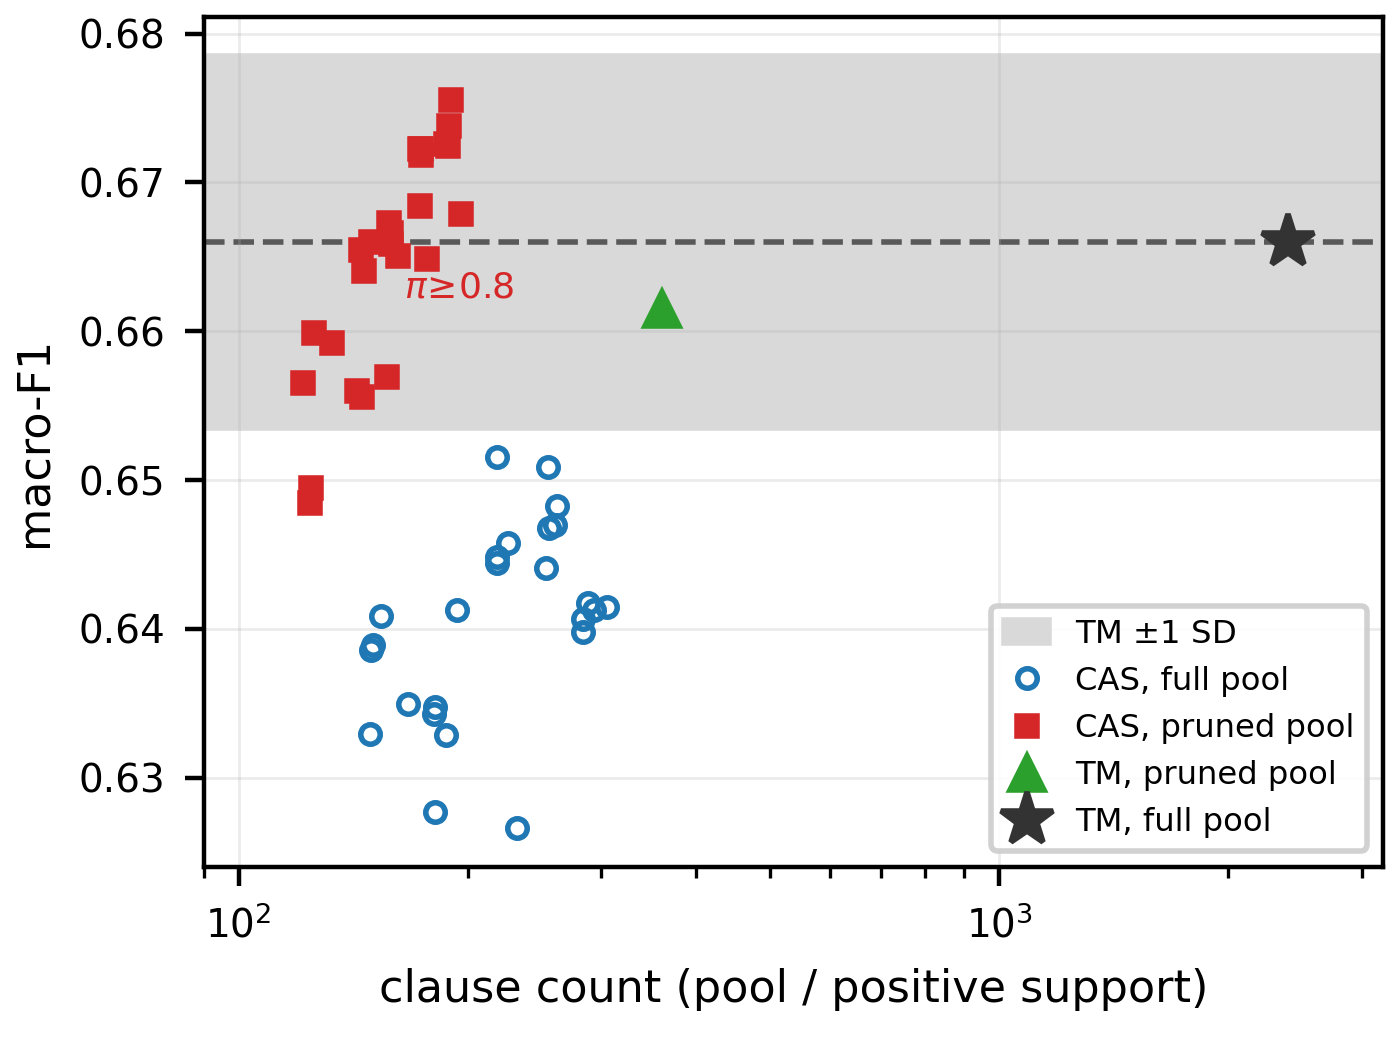
\includegraphics[width=\columnwidth]{fig_signature_frontier.png}
\caption{Retained macro-F1 against signature size on the report set.
Each marker is one $(B,\pi_{\mathrm{thr}})$ operating point. The band
is the full TM's seed spread. Pruned-pool signatures of 122--196
clauses stay within that band, against 2,400 clauses for the full TM.}
\label{fig:frontier}
\end{figure}

\subsection{Sensitivity Before and After Pruning}
\label{sec:sweep}
At $B=15$, sweeping $\pi_{\mathrm{thr}}$ over
$\{0.5,\ldots,0.9\}$ spans macro-F1 0.656--0.674 on the pruned pool and
0.633--0.652 on the full pool. At $\pi_{\mathrm{thr}}=0.8$, varying $B$
from 5 to 25 spans 0.656--0.666 and 0.628--0.641 respectively.
Figure~\ref{fig:sweep} shows both sweeps against the pruned-TM
baselines. The pruned pool stays inside the TM's seed spread throughout,
while the full pool stays below it. The pruned pool is therefore the
regime in which the signature preserves the detector's accuracy.
Figure~\ref{fig:frontier} gives the corresponding signature sizes.
Every pruned-pool operating point lies between 122 and 196 clauses.

\begin{figure}[t]
\centering
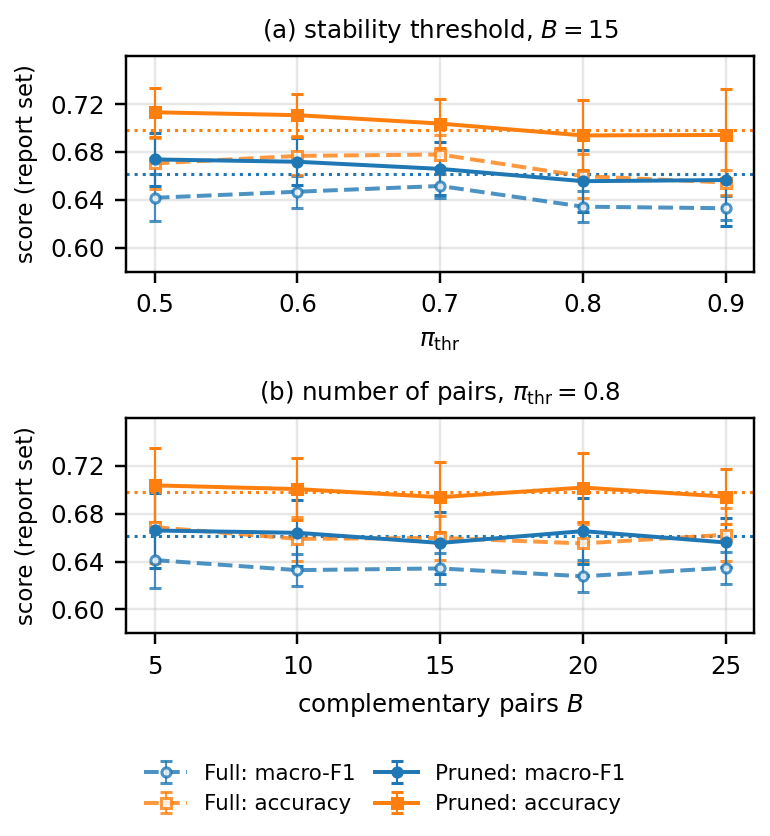
\includegraphics[width=\columnwidth]{fig_sweep_heldout.png}
\caption{Full (dashed, open markers) and pruned (solid, filled) CAS,
report-set mean$\pm$SD over three seeds: (a) threshold sweep at $B=15$;
(b) pair-count sweep at $\pi_{\mathrm{thr}}=0.8$. Dotted lines show the
pruned-TM baselines.}
\label{fig:sweep}
\end{figure}


\subsection{Pruning and Signature Size}
\label{sec:pruned}\label{sec:signatures}
Figure~\ref{fig:pruning} sweeps the removal budget. Report-set
macro-F1 and accuracy stay flat from the full 2,400-clause pool down to
roughly 360 clauses and fall away only under more aggressive removal.
The magnitude rule reads the selection partition alone and chooses
$k^*=340$, leaving 60 clauses per class and 360 in total, a reduction
of $85\%$. At that budget the pruned TM achieves macro-F1
$0.6615\pm0.0115$ against $0.6660\pm0.0125$ for the full pool
(Table~\ref{tab:headline}), so weight-based pruning alone removes
six-sevenths of the pool at no measurable cost.

\begin{figure}[t]
\centering
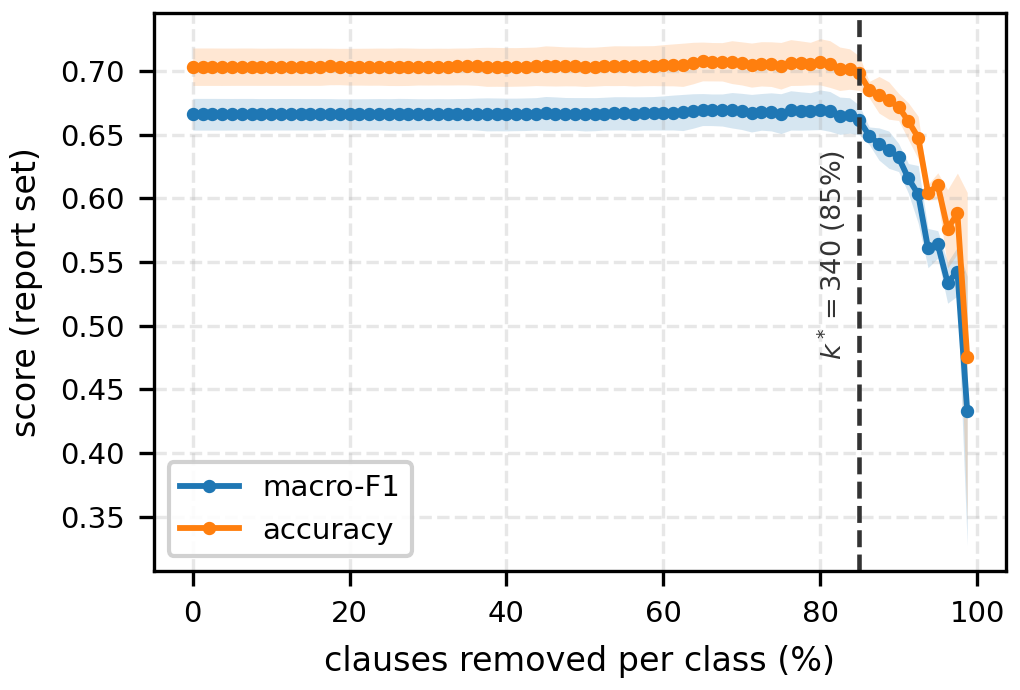
\includegraphics[width=0.92\columnwidth]{fig_clause_pruning_heldout.png}
\caption{Report-set pruning sensitivity (three-seed mean$\pm$SD). The
budget $k^*=340$, chosen on the separate selection partition, is marked
by the dashed line. Scores are flat until roughly that point.}
\label{fig:pruning}
\end{figure}

Applying CPSS to the retained 360-clause pool reduces the evidence
further. At $\pi_{\mathrm{thr}}=0.8$ the signature holds 149 clauses
and matches the full TM. Raising the threshold to $0.9$ leaves 126.
Relative to the 2,400-clause pool this is a $16$--$19\times$ reduction.
Weight pruning contributes $6.7\times$ of it, and CPSS the remainder.

Table~\ref{tab:reduction} lists per-class positive-evidence supports
$|S^+|$ for seed 42 at each pool's selected operating point. The
distribution is uneven. Spoofing retains the largest support in both
pools, while MQTT falls to 17 clauses on the pruned pool. Rerunning
CPSS on the retained pool therefore redistributes the selected evidence
across families rather than shrinking each signature proportionally.

\begin{table}[!htb]
\centering
\caption{Per-class positive-evidence support $|S^+|$ at each pool's
selected operating point, seed 42.}
\label{tab:reduction}
\footnotesize
\begin{tabular}{@{}lcc@{}}
\toprule
Class & Full pool (2,400) & Pruned pool (360) \\
\midrule
Benign & 21 & 35 \\
DDoS & 29 & 29 \\
DoS & 21 & 38 \\
MQTT & 21 & 17 \\
Recon & 19 & 27 \\
Spoofing & 39 & 39 \\
\midrule
Total & 150 & 185 \\
\bottomrule
\end{tabular}
\end{table}

\section{Conclusion}
Clause-Activation Signatures (CAS) convert a trained weighted Tsetlin
Machine's clause pool into signed evidence for IoMT attack-family
attribution. CPSS selects recurring clauses, averaged coefficient signs
distinguish supporting from opposing evidence, and optional weight-based
pruning reduces the candidate pool. We derive a sufficient margin
condition for preserving TM predictions after pruning. The CPSS bound
controls low-selection-probability inclusions under its sampling
conditions; it does not by itself certify false discoveries or evidence signs.

On capped CICIoMT2024 WiFi/MQTT data the full 2,400-clause TM reaches
mean multiclass macro-F1 $0.6660\pm0.0125$ across three seeds. Weight
pruning removes $85\%$ of the pool at no measurable cost. CPSS then
reduces the retained evidence to 149 clauses at
$\pi_{\mathrm{thr}}=0.8$, with macro-F1 $0.6660\pm0.0316$, or to 126
clauses at $\pi_{\mathrm{thr}}=0.9$. The signature is thus
$16$--$19\times$ smaller than the clause pool it summarises, while
accuracy is unchanged. A decision tree, an $\ell_1$ linear model,
XGBoost and a random forest on the same literals span $0.6551$ to
$0.6948$. CAS is competitive with these models rather than superior,
and its contribution is the form of its output. Two ablations support
that reading. Substituting the input literals for the clause pool under
the same readout costs $0.078$ macro-F1. A sign-agnostic scorer
collapses to $0.025$. Both the conjunctive structure of the clauses and
their coefficient signs are therefore load-bearing. Reliance on one
capped dataset, and the absence of a deployment-time study, require
independent validation before deployment claims.
%\clearpage
\bibliographystyle{IEEEtran}
\bibliography{CAS_4page}
\end{document}
